\chapter{RESULTADOS DE SIMULAÇÕES}
\label{resultados}
\section{\textbf{Introdução}}
Neste capítulo serão apresentadas as simulações realizadas para analisar o comportamento de partículas presentes em turbomáquinas em ação.
Foram escolhidos quatro tipos de geometria para serem simulados:
\begin{itemize}
    \item \textbf{Canal reto}.

        Uma geometria simples, que busca simular o comportamento básico das partículas sobre efeito de um escoamento. 
        A malha utilizada tem $1072$ elementos definidos sobre $593$ nós, exposta na \ref{channel_mesh}.
        \begin{figure}[H]
            \centering
            \stackunder{
                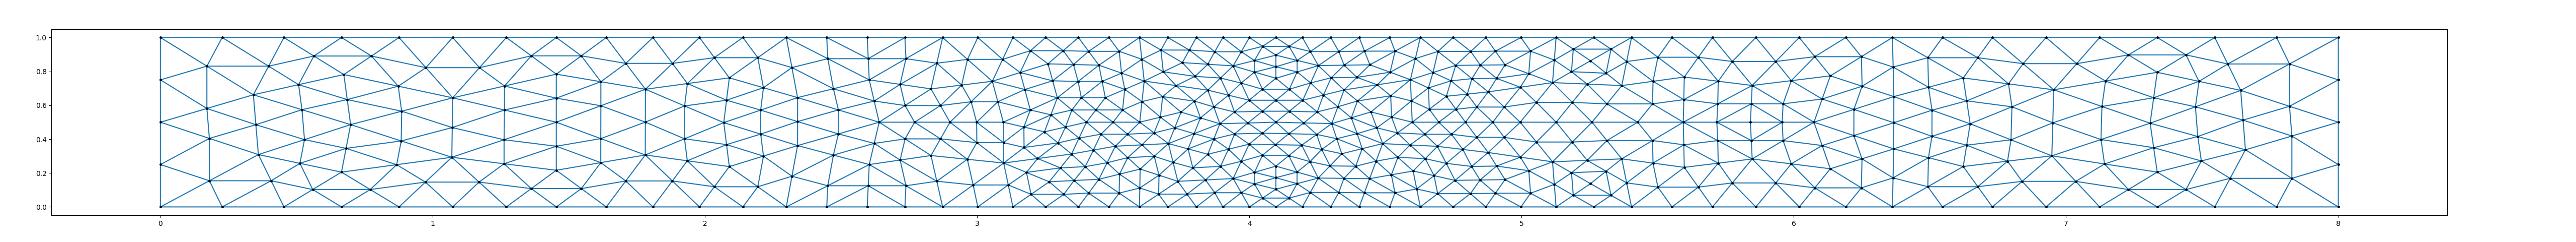
\includegraphics[width=\linewidth]{figures/Channel_mesh.png}
            } {\raggedleft \scriptsize Fonte: Autor.}
            \caption{Malha da simulação em um canal reto.}
            \label{channel_mesh}
        \end{figure}

    \item \textbf{Canal com um obstáculo circular no centro}.

        Esta geometria visa simular o efeito de obstáculos, ou até mesmo as próprias partículas no escoamento.
        Porém, não é utilizada neste trabalho a implementação \textit{two-way}, que levaria em conta os efeitos das partículas no escoamento.
        Neste caso a simulação foi aplicada a uma malha de $868$ elementos e $494$ nós.
        \begin{figure}[H]
            \centering
            \stackunder{
                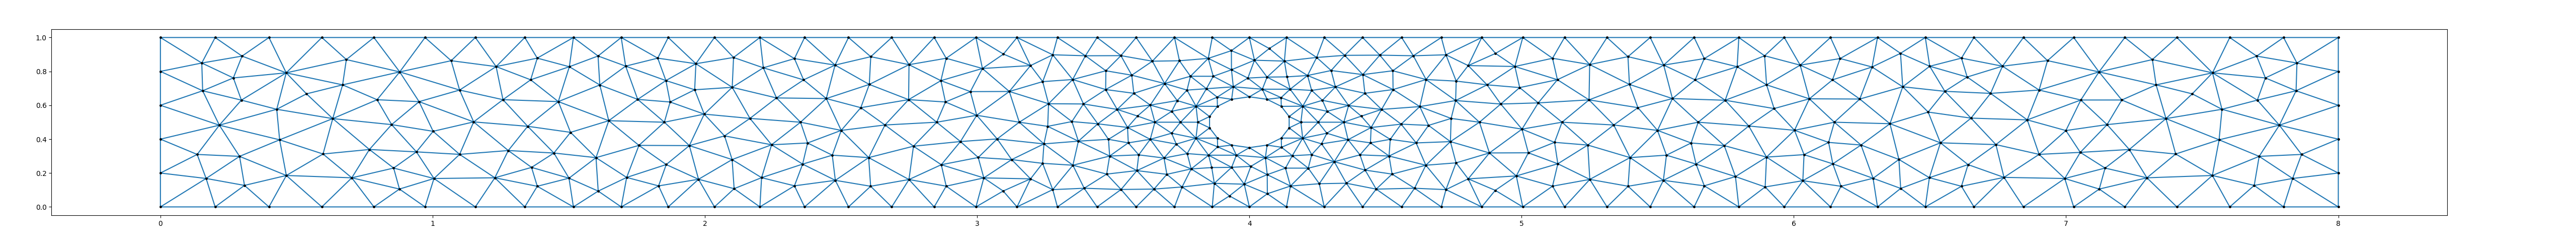
\includegraphics[width=\linewidth]{figures/Obstacle_mesh.png}
            } {\raggedleft \scriptsize Fonte: Autor.}
            \caption{Malha da simulação em um canal com um obstáculo.}
            \label{obstacle_mesh}
        \end{figure}

    \item \textbf{Canal com degrau}.

        O escoamento em um canal com um degrau, ou uma diferença brusca de percurso, possui diversos efeitos interessantes para serem observados.
        Como por exemplo as regiões 
        Com uma malha de $676$ elementos definidos sobre $380$ nós.
        \begin{figure}[H]
            \centering
            \stackunder{
                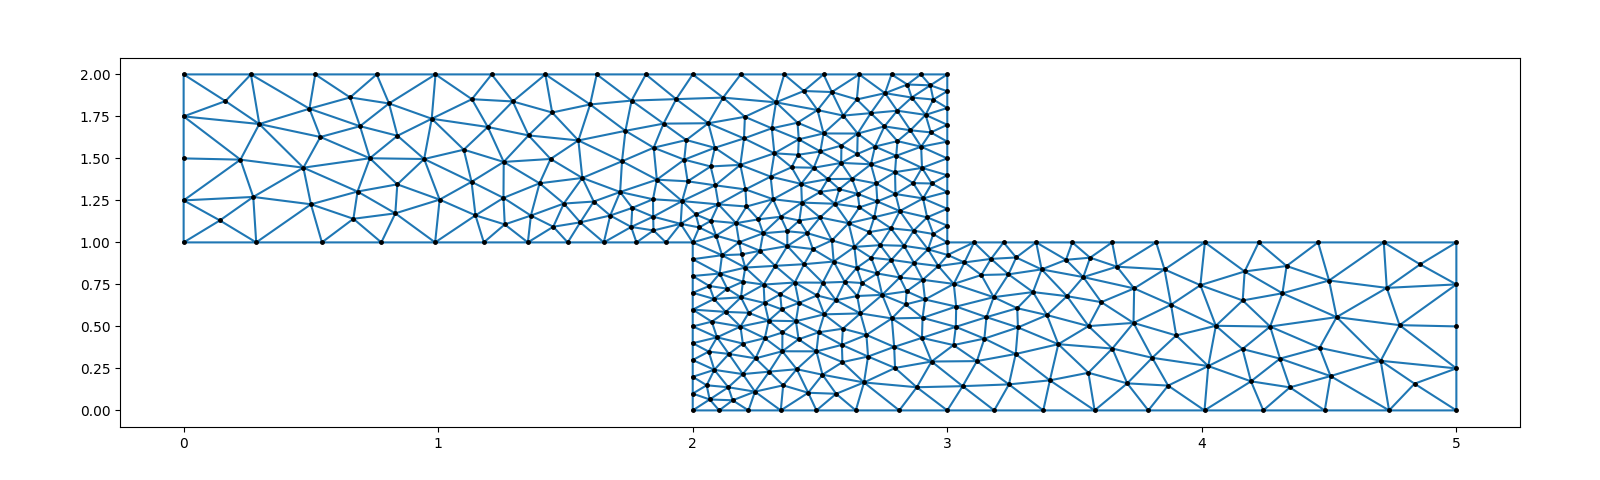
\includegraphics[width=\linewidth]{figures/Step_mesh.png}
            } {\raggedleft \scriptsize Fonte: Autor.}
            \caption{Malha da simulação em um canal com degrau.}
            \label{step_mesh}
        \end{figure}

    \item \textbf{Pá de um rotor}.

        Finalmente, será analizado o comportamento de partículas em um escoamento presente em uma seção de um rotor de uma turbomáquina.
        Neste trabalho, foi tomado um referencial estacionário na pá, sem efeito da rotação do rotor no escoamento.
        Foi utilizada uma malha de $1058$ elementos definidos sobre $531$ nós.
        \begin{figure}[H]
            \centering
            \stackunder{
                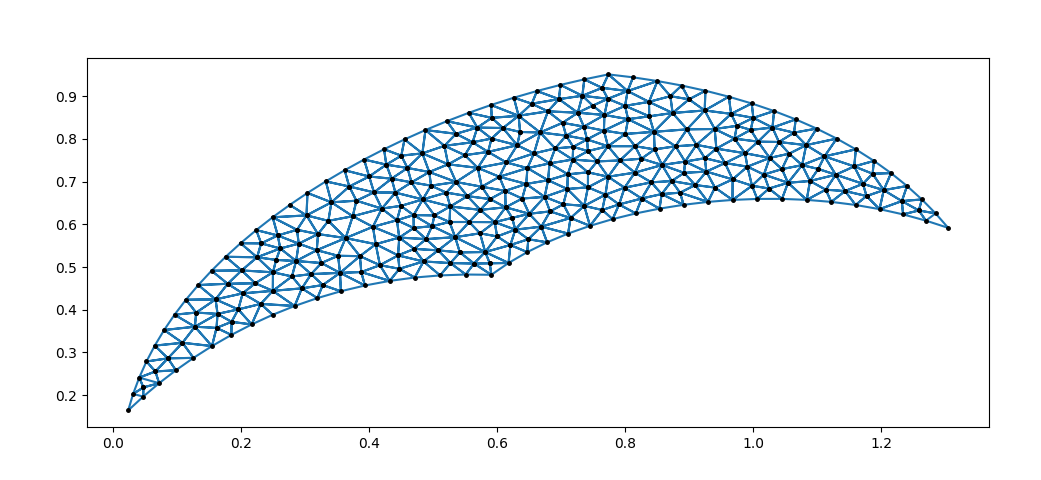
\includegraphics[width=\linewidth]{figures/Rotor_mesh.png}
            } {\raggedleft \scriptsize Fonte: Autor.}
            \caption{Malha da simulação em uma pá de um rotor.}
            \label{rotor_mesh}
        \end{figure}
\end{itemize}

Foi utilizado o software ParaView\cite{paraview} para exibição dos gráficos de resultados.
A escala das figuras mostra o valor da magnitude da velocidade em cada nó.

Em cada simulação são aplicadas partículas perfeitamente rígidas, igualmente espalhadas, com $d_p=1mm=1.10^{-3}m$ de diâmetro e densidade de $\rho_p=30000kg/m^3$.
Estas partículas estão submersas em um fluido ideal com características 

%------------------- Canal Reto--------------------------------
\section{\textbf{Simulação Em Um Canal Reto}}
\label{sec_channel_reto}
O escoamento em um canal reto permite vizualizar o movimento livre das partículas sob efeito do fluido.
A sua configuração é similar ao exemplo de Poiseuille \ref{sec_poiseuille}.
Seu campo de velocidades é apresentado na \ref{channel_result}:
\begin{figure}[H]
    \centering
    \stackunder{
        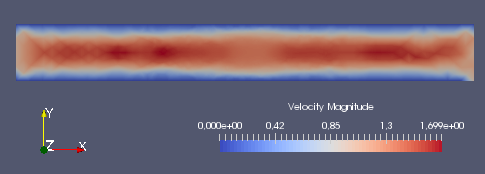
\includegraphics[width=\linewidth]{figures/Channel_result.png}
    } {\raggedleft \scriptsize Fonte: Autor.}
    \caption{Campo de velocidades de um escoamento em um canal reto.}
    \label{channel_result}
\end{figure}


%------------------- Obstaculo --------------------------------
\section{\textbf{Simulação Em Um Canal Com Obtáculo}}
\label{sec_obstacle}
Em um escoamento com obtáculo, pode-se observar o efeito do obstáculo no campo de velocidades do escoamento, assim como o comportamento das partículas ao interagir com este obstáculo.
Para auxiliar na visualização do resultado, é exibido em conjunto da velocidade as linhas de corrente do campo, desenhadas com o auxílio de uma ferramenta de desenho das curvas de nível.
Observa-se a distorção no campo de velocidades causada pelo obstáculo na \ref{obstacle_result}:
\begin{figure}[H]
    \centering
    \stackunder{
        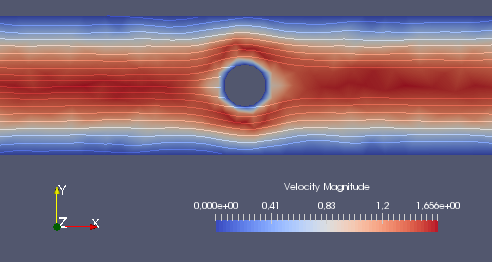
\includegraphics[width=\linewidth]{figures/Obstacle_result.png}
    } {\raggedleft \scriptsize Fonte: Autor.}
    \caption{Campo de velocidades de um escoamento com obstáculo.}
    \label{obstacle_result}
\end{figure}


%------------------- Step ------------------------------------
\section{\textbf{Simulação Em Um Canal Com Degrau}}
\label{sec_step}
No escoamento com degrau há um desvio no trajeto que tende a causar colisões das partículas devio a inércia de seu movimento.
Dependendo de suas características, as partículas estão mais propensas a colidirem com a parede direita superior ou serão mais influenciadas pelo fluido e terão sua trajetória alterada.
Novamente, são incluidas as curvas de nível da velocidade na exibição do campo de velocidades na \ref{step_result}:
\begin{figure}[H]
    \centering
    \stackunder{
        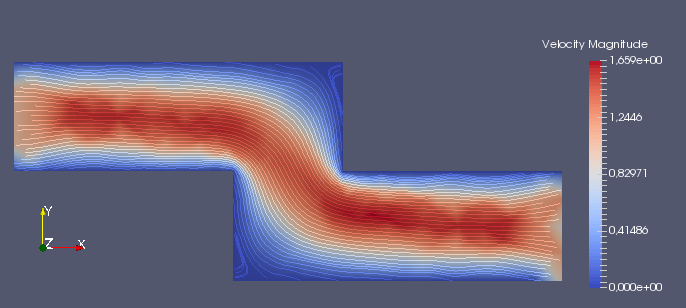
\includegraphics[width=\linewidth]{figures/Step_result.png}
    } {\raggedleft \scriptsize Fonte: Autor.}
    \caption{Campo de velocidades de um escoamento com degrau.}
    \label{step_result}
\end{figure}

Como outra forma de visualizar o campo de velocidades, são exibidas as velocidades nos nós como vetores em um diagrama de flechas ou \textit{quiver plot}:
\begin{figure}[H]
    \centering
    \stackunder{
        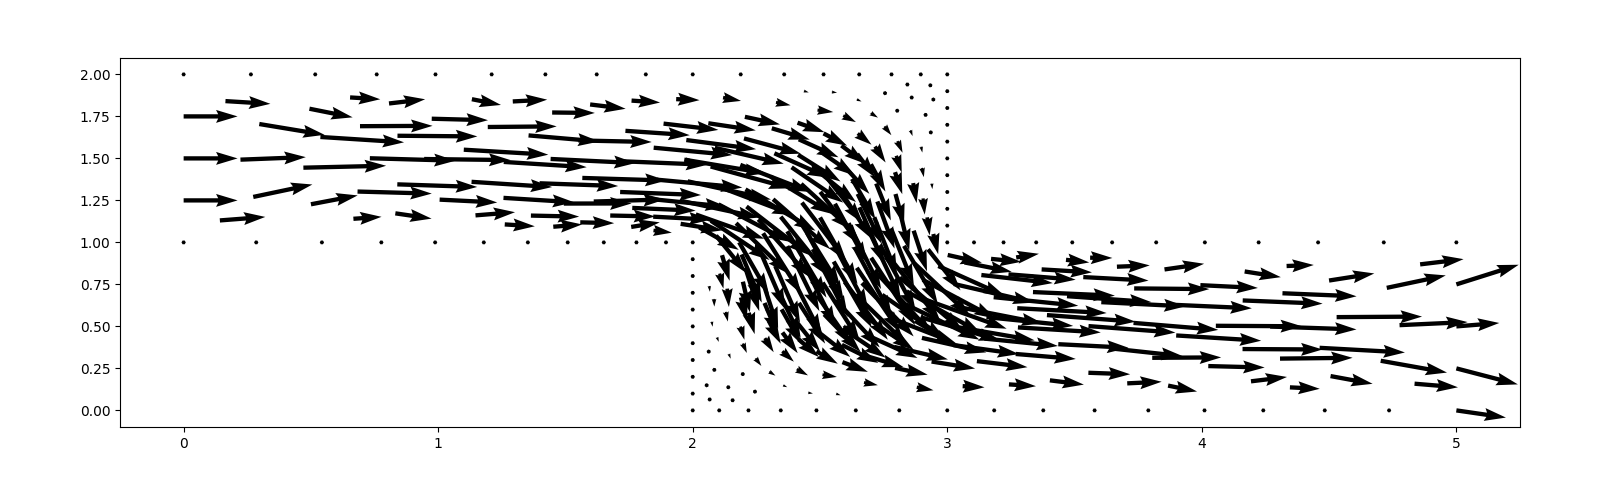
\includegraphics[width=\linewidth]{figures/Step_velocity_field.png}
    } {\raggedleft \scriptsize Fonte: Autor.}
    \caption{Vetores de velocidades de um escoamento com degrau.}
    \label{step_velocity}
\end{figure}


%------------------- Step ------------------------------------
\section{\textbf{Simulação Em Uma Pá de Rotor}}
\label{sec_rotor}
Finalmente, a simulação em uma pá de rotor visa representar o comportamento das partículas em uma situação real de trabalho de uma trubomáquina.

Neste trabalho, não serão levadas em conta as forças provenientes da rotação da máquina.
Portanto, é assumido que o domínio presente da pá é estacionário e é tomado como referência.

Novamente, são incluidas as curvas de nível da velocidade na exibição do campo de velocidades na \ref{rotor_result}:
\begin{figure}[H]
    \centering
    \stackunder{
        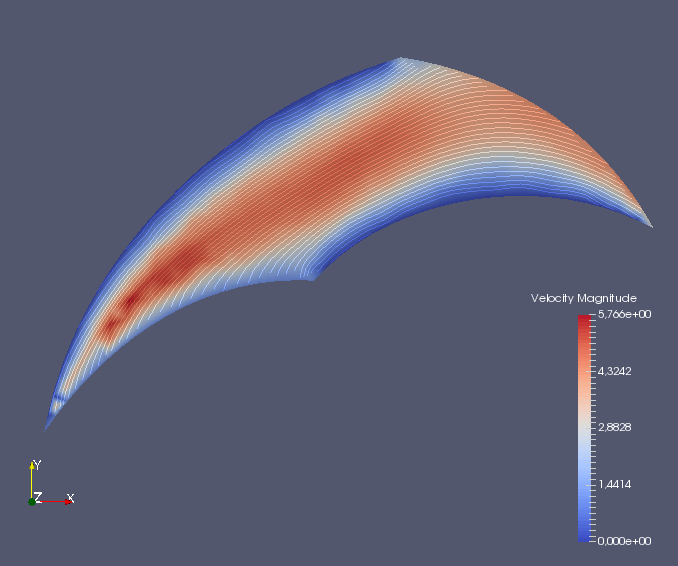
\includegraphics[width=\linewidth]{figures/Rotor_result.png}
    } {\raggedleft \scriptsize Fonte: Autor.}
    \caption{Campo de velocidades de um escoamento em uma pá de um rotor.}
    \label{rotor_result}
\end{figure}

E os vetores das velocidades nos nós:
\begin{figure}[H]
    \centering
    \stackunder{
        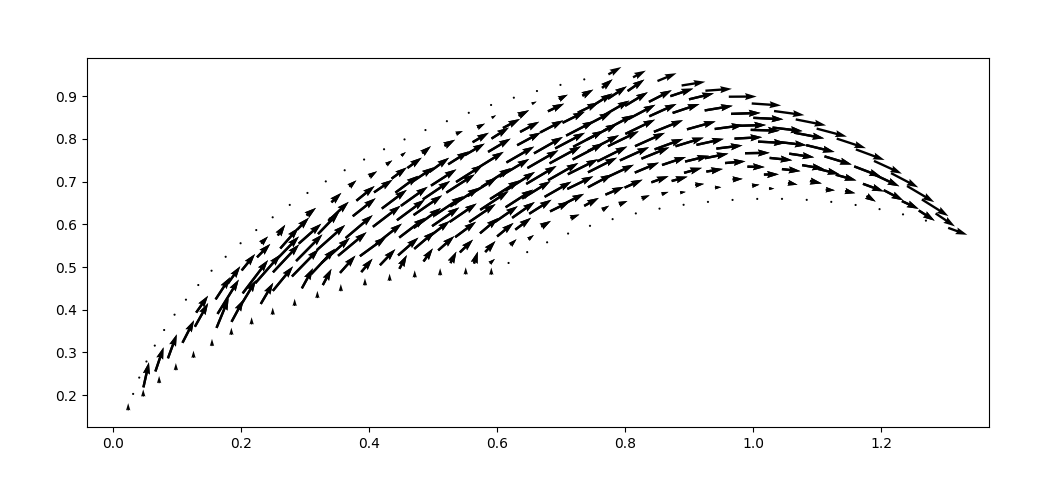
\includegraphics[width=\linewidth]{figures/Rotor_velocity_field.png}
    } {\raggedleft \scriptsize Fonte: Autor.}
    \caption{Vetores de velocidades de um escoamento em uma pá de um rotor.}
    \label{rotor_velocity}
\end{figure}